\documentclass[11pt,a4paper]{article}

% ============================================
% PAQUETES
% ============================================
\usepackage[utf8]{inputenc}
\usepackage[spanish, provide=*]{babel}
\usepackage[T1]{fontenc}
\usepackage{geometry}
\usepackage{graphicx}
\usepackage{float}
\usepackage{booktabs}
\usepackage{longtable}
\usepackage{array}
\usepackage{multirow}
\usepackage{amsmath}
\usepackage{amssymb}
\usepackage{hyperref}
\usepackage{listings}
\usepackage{xcolor}
\usepackage{fancyhdr}
\usepackage{titlesec}
\usepackage{caption}
\usepackage{subcaption}
\usepackage{enumitem}
\usepackage{tikz}
\usetikzlibrary{shapes.geometric, arrows, positioning, fit, backgrounds}

% ============================================
% CONFIGURACIÓN DE PÁGINA
% ============================================
\geometry{
    left=2.2cm,
    right=2.2cm,
    top=2.2cm,
    bottom=2.2cm
}

% ============================================
% CONFIGURACIÓN DE COLORES
% ============================================
\definecolor{codegreen}{rgb}{0,0.6,0}
\definecolor{codegray}{rgb}{0.5,0.5,0.5}
\definecolor{codepurple}{rgb}{0.58,0,0.82}
\definecolor{backcolour}{rgb}{0.95,0.95,0.92}
\definecolor{primaryblue}{RGB}{41, 98, 255}

% ============================================
% CONFIGURACIÓN DE CÓDIGO
% ============================================
\lstdefinestyle{mystyle}{
    backgroundcolor=\color{backcolour},   
    commentstyle=\color{codegreen},
    keywordstyle=\color{magenta},
    numberstyle=\tiny\color{codegray},
    stringstyle=\color{codepurple},
    basicstyle=\ttfamily\footnotesize,
    breakatwhitespace=false,         
    breaklines=true,                 
    captionpos=b,                    
    keepspaces=true,                 
    numbers=left,                    
    numbersep=5pt,                  
    showspaces=false,                
    showstringspaces=false,
    showtabs=false,                  
    tabsize=2
}
\lstset{style=mystyle}

% ============================================
% CONFIGURACIÓN DE ENCABEZADOS
% ============================================
\pagestyle{fancy}
\fancyhf{}
\rhead{MHealth HAR}
\lhead{Proyecto Final}
\rfoot{Página \thepage}

% ============================================
% INFORMACIÓN DEL DOCUMENTO
% ============================================
\title{
    \vspace{-1cm}
    \textbf{Sistema de Reconocimiento de Actividad Humana}\\
    \large Basado en el Dataset MHealth\\
    \vspace{0.5cm}
    \normalsize Proyecto Final - Despliegue de Modelos de Machine Learning
}
\author{
    Universidad\\
    Curso: Taller Final
}
\date{Diciembre 2025}

% ============================================
% INICIO DEL DOCUMENTO
% ============================================
\begin{document}

\maketitle
\thispagestyle{empty}

% ============================================
% RESUMEN
% ============================================
\begin{abstract}
    Este documento presenta el desarrollo e implementación de un sistema completo de Reconocimiento de Actividad Humana (HAR) utilizando el dataset MHealth. El sistema integra un pipeline de Machine Learning reproducible, una API REST desarrollada con FastAPI y una interfaz web moderna construida con React y TypeScript. El modelo Random Forest implementado alcanza un accuracy del 92.6\% y un Macro F1-Score del 92.6\% en validación, permitiendo clasificar 12 actividades físicas diferentes a partir de señales de sensores corporales. La arquitectura del sistema sigue principios de diseño modular, facilitando el mantenimiento, la escalabilidad y el despliegue mediante contenedores Docker.
\end{abstract}

\vspace{0.5cm}
\textbf{Palabras clave:} Reconocimiento de Actividad Humana, Machine Learning, FastAPI, React, MHealth, Series Temporales, Random Forest.

\newpage
\tableofcontents
\newpage

% ============================================
% 1. INTRODUCCIÓN
% ============================================
\section{Introducción}

\subsection{Contexto del Problema}

El reconocimiento de actividad humana (HAR, por sus siglas en inglés \textit{Human Activity Recognition}) constituye un área de investigación fundamental en el campo de la computación ubicua y el aprendizaje automático. Esta disciplina tiene aplicaciones directas en salud digital, monitoreo de pacientes, deportes, rehabilitación física y sistemas de asistencia inteligente.

El presente proyecto surge como fase final de un curso donde se trabajó iterativamente con el dataset MHealth, abordando desde la obtención y exploración de datos hasta el modelado y evaluación de algoritmos. Esta etapa final corresponde al \textbf{despliegue}, integrando el modelo entrenado en un sistema funcional compuesto por backend, frontend y documentación completa.

\subsection{Objetivo General}

Desarrollar y desplegar una aplicación web completa para reconocimiento de actividad humana que:

\begin{itemize}[noitemsep]
    \item Integre un modelo de clasificación entrenado sobre el dataset MHealth
    \item Exponga una API REST para realizar predicciones
    \item Ofrezca una interfaz de usuario accesible para usuarios no técnicos
    \item Incluya instrucciones de despliegue y uso reproducibles
    \item Documente el uso de herramientas de IA generativa
\end{itemize}

\subsection{Objetivos Específicos}

\begin{enumerate}[noitemsep]
    \item Implementar un pipeline de preprocesamiento que transforme señales crudas en características estadísticas por ventana temporal
    \item Entrenar y evaluar un modelo de clasificación que distinga entre 12 actividades físicas
    \item Desarrollar un backend RESTful que permita predicción y evaluación de archivos \texttt{.log}
    \item Construir un frontend moderno que visualice predicciones y métricas de manera intuitiva
    \item Containerizar la aplicación para facilitar su despliegue y reproducibilidad
\end{enumerate}

% ============================================
% 2. DATASET Y PREPROCESAMIENTO
% ============================================
\section{Dataset y Preprocesamiento}

\subsection{Descripción del Dataset MHealth}

El dataset MHealth (\textit{Mobile Health}) fue recolectado por la Universidad Politécnica de Cataluña y está disponible públicamente en el repositorio UCI Machine Learning Repository\footnote{\url{https://archive.ics.uci.edu/dataset/319/mhealth+dataset}}. Contiene registros de 10 sujetos realizando 12 actividades físicas diferentes mientras portaban sensores corporales.

\subsubsection{Características de los Sensores}

Se utilizan tres dispositivos de medición inercial ubicados en:
\begin{itemize}[noitemsep]
    \item \textbf{Pecho:} Acelerómetro (3 ejes) + 2 canales ECG
    \item \textbf{Tobillo izquierdo:} Acelerómetro, giroscopio y magnetómetro (3 ejes c/u)
    \item \textbf{Brazo derecho:} Acelerómetro, giroscopio y magnetómetro (3 ejes c/u)
\end{itemize}

En total, cada muestra contiene \textbf{23 columnas de sensores} más la etiqueta de actividad. La frecuencia de muestreo es de \textbf{50 Hz}.

\subsubsection{Actividades Clasificadas}

El sistema reconoce 12 actividades: De pie (1), Sentado (2), Acostado (3), Caminando (4), Subiendo escaleras (5), Flexión de cintura (6), Elevación frontal de brazos (7), Flexión de rodillas (8), Ciclismo (9), Trote (10), Corriendo (11) y Saltando (12).

\subsection{Pipeline de Preprocesamiento}

Las señales se segmentan en ventanas deslizantes de \textbf{5 segundos} con \textbf{50\% de solapamiento}. Para cada ventana y sensor, se extraen 7 características estadísticas: media, desviación estándar, mínimo, máximo, mediana, MAD y energía, generando $23 \times 7 = \textbf{161 características}$ por ventana. Se aplica normalización Z-score ajustada exclusivamente sobre datos de entrenamiento.

\subsection{Manejo del Desbalance de Clases}

El dataset original incluye una \textbf{actividad 0} (``Sin clasificar'') que constituye el 93\% de las muestras. Se filtran todas las muestras con actividad 0 durante el preprocesamiento, ya que no representa una actividad física significativa y su predominancia impedía el aprendizaje de patrones útiles.

% ============================================
% 3. ARQUITECTURA DEL SISTEMA
% ============================================
\section{Arquitectura del Sistema}

\subsection{Visión General}

El sistema sigue una arquitectura de tres capas claramente separadas: capa de Machine Learning, capa de Backend (API) y capa de Frontend (UI). La Figura~\ref{fig:arquitectura} ilustra la interacción entre componentes.

\begin{figure}[H]
    \centering
    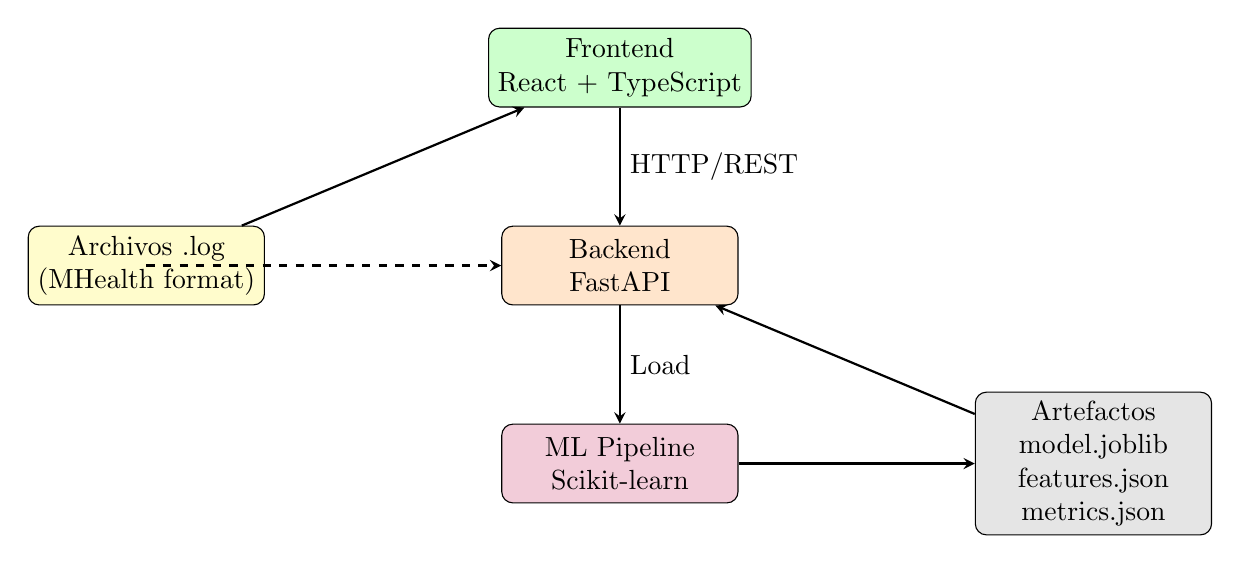
\begin{tikzpicture}[
            node distance=1.5cm,
            box/.style={rectangle, draw, rounded corners, minimum width=3cm, minimum height=1cm, align=center, fill=blue!10},
            arrow/.style={->, thick, >=stealth}
        ]

        % Frontend
        \node[box, fill=green!20] (frontend) {Frontend\\React + TypeScript};

        % Backend
        \node[box, fill=orange!20, below=of frontend] (backend) {Backend\\FastAPI};

        % ML Pipeline
        \node[box, fill=purple!20, below=of backend] (ml) {ML Pipeline\\Scikit-learn};

        % Artifacts
        \node[box, fill=gray!20, right=3cm of ml] (artifacts) {Artefactos\\model.joblib\\features.json\\metrics.json};

        % Database (archivos)
        \node[box, fill=yellow!20, left=3cm of backend] (files) {Archivos .log\\(MHealth format)};

        % Conexiones
        \draw[arrow] (frontend) -- node[right] {HTTP/REST} (backend);
        \draw[arrow] (backend) -- node[right] {Load} (ml);
        \draw[arrow] (ml) -- (artifacts);
        \draw[arrow] (artifacts) -- (backend);
        \draw[arrow] (files) -- (frontend);
        \draw[arrow, dashed] (files) |- (backend);

    \end{tikzpicture}
    \caption{Arquitectura general del sistema MHealth HAR}
    \label{fig:arquitectura}
\end{figure}

\subsection{Estructura del Repositorio}

El proyecto está organizado como un monorepo con tres componentes principales:
\begin{itemize}[noitemsep]
    \item \texttt{ml/}: Pipeline de datos y scripts de entrenamiento/evaluación
    \item \texttt{backend/}: Servicio FastAPI con endpoints y lógica de negocio
    \item \texttt{frontend/}: Aplicación React con TypeScript
    \item \texttt{config/}: Configuración centralizada (YAML)
    \item \texttt{prompts/}: Documentación de uso de IA generativa
\end{itemize}


% ============================================
% 4. MODELO DE MACHINE LEARNING
% ============================================
\section{Modelo de Machine Learning}

\subsection{Selección del Algoritmo}

Se seleccionó \textbf{Random Forest Classifier} por las siguientes razones:

\begin{enumerate}[noitemsep]
    \item \textbf{Robustez:} Maneja bien características correlacionadas y no requiere supuestos distribucionales
    \item \textbf{Interpretabilidad:} Permite analizar importancia de features
    \item \textbf{Eficiencia:} Entrenamiento rápido y paralelizable
    \item \textbf{Generalización:} El ensemble de árboles reduce overfitting
    \item \textbf{Balance de clases:} Soporta nativamente pesos por clase
\end{enumerate}

\subsection{Hiperparámetros}

\begin{table}[H]
    \centering
    \caption{Configuración del modelo Random Forest}
    \label{tab:hiperparametros}
    \begin{tabular}{ll}
        \toprule
        \textbf{Parámetro} & \textbf{Valor}       \\
        \midrule
        n\_estimators      & 200                  \\
        max\_depth         & None (sin límite)    \\
        class\_weight      & balanced             \\
        random\_state      & 42                   \\
        n\_jobs            & -1 (todos los cores) \\
        \bottomrule
    \end{tabular}
\end{table}

\subsection{División de Datos}

Para garantizar la ausencia de fuga de datos, la división se realiza \textbf{por sujeto}, no por muestra. Esto asegura que las ventanas de un mismo sujeto no aparezcan simultáneamente en conjuntos de entrenamiento y evaluación.

\begin{table}[H]
    \centering
    \caption{División de sujetos para entrenamiento y evaluación}
    \label{tab:splits}
    \begin{tabular}{lll}
        \toprule
        \textbf{Conjunto} & \textbf{Sujetos} & \textbf{Proporción} \\
        \midrule
        Entrenamiento     & 4, 5, 6, 10      & 60\%                \\
        Validación        & 3, 9             & 20\%                \\
        Test              & 2, 7             & 20\%                \\
        Demo (excluidos)  & 1, 8             & ---                 \\
        \bottomrule
    \end{tabular}
\end{table}

Los sujetos 1 y 8 fueron completamente excluidos del entrenamiento, validación y normalización. Estos sujetos sirven como conjunto de demostración para validar el sistema end-to-end en la interfaz web.

\subsection{Resultados y Métricas}

\begin{table}[H]
    \centering
    \caption{Métricas de rendimiento del modelo}
    \label{tab:metricas}
    \begin{tabular}{lcc}
        \toprule
        \textbf{Conjunto}   & \textbf{Accuracy} & \textbf{Macro F1-Score} \\
        \midrule
        Entrenamiento       & 100.0\%           & 100.0\%                 \\
        Validación          & 92.6\%            & 92.6\%                  \\
        Test                & 81.3\%            & 81.1\%                  \\
        Demo (sujetos 1, 8) & 99.3\%            & 99.1\%                  \\
        \bottomrule
    \end{tabular}
\end{table}

El alto rendimiento en el conjunto Demo indica que el modelo generaliza correctamente a sujetos no vistos durante el entrenamiento.

\subsection{Impacto de la Eliminación de Actividad 0}

La Tabla~\ref{tab:mejoras} compara el rendimiento antes y después de filtrar la actividad 0:

\begin{table}[H]
    \centering
    \caption{Comparación de métricas antes y después de filtrar actividad 0}
    \label{tab:mejoras}
    \begin{tabular}{lcccc}
        \toprule
        \textbf{Métrica} & \textbf{Antes} & \textbf{Después} & \textbf{$\Delta$ Absoluto} & \textbf{$\Delta$ Relativo} \\
        \midrule
        Accuracy (Val)   & 71.8\%         & 92.6\%           & +20.8\%                    & +29.0\%                    \\
        Macro F1 (Val)   & 13.7\%         & 92.6\%           & +78.9\%                    & +575.9\%                   \\
        Accuracy (Test)  & 73.9\%         & 81.3\%           & +7.4\%                     & +10.0\%                    \\
        Macro F1 (Test)  & 12.0\%         & 81.1\%           & +69.1\%                    & +575.8\%                   \\
        \bottomrule
    \end{tabular}
\end{table}

% ============================================
% 5. BACKEND - API REST
% ============================================
\section{Backend - API REST}

\subsection{Tecnologías Utilizadas}

\begin{itemize}[noitemsep]
    \item \textbf{FastAPI:} Framework web moderno, de alto rendimiento, con validación automática y documentación OpenAPI
    \item \textbf{Pydantic v2:} Validación de datos y serialización
    \item \textbf{Uvicorn:} Servidor ASGI para producción
    \item \textbf{Python 3.11+:} Lenguaje base
\end{itemize}

\subsection{Endpoints de la API}

\begin{table}[H]
    \centering
    \caption{Descripción de endpoints de la API}
    \label{tab:endpoints}
    \begin{tabular}{llp{7cm}}
        \toprule
        \textbf{Método} & \textbf{Endpoint} & \textbf{Descripción}                                                                              \\
        \midrule
        GET             & /health           & Verifica que el servicio está activo. Retorna \texttt{\{``status'': ``ok''\}}                     \\
        GET             & /model-info       & Retorna información del modelo: versión, hiperparámetros, métricas de entrenamiento, sujetos demo \\
        POST            & /predict          & Recibe archivo .log y retorna predicción por ventana con probabilidades                           \\
        POST            & /evaluate-log     & Recibe archivo .log etiquetado y retorna métricas (accuracy, F1, matriz de confusión)             \\
        \bottomrule
    \end{tabular}
\end{table}

\subsection{Formato de Entrada y Salida}

\begin{itemize}[noitemsep]
    \item \textbf{POST /predict:} Recibe archivo \texttt{.log} (23 columnas). Retorna JSON con predicción por ventana (índice, actividad, probabilidades) y resumen agregado (distribución por actividad).
    \item \textbf{POST /evaluate-log:} Recibe archivo \texttt{.log} etiquetado (24 columnas). Retorna métricas (accuracy, macro\_f1), matriz de confusión, predicciones y ground truth.
\end{itemize}

El detalle completo de los esquemas JSON se encuentra en el documento de anexos.

\subsection{Manejo de Errores}

La API implementa validación de entrada y retorna códigos HTTP apropiados:

\begin{itemize}[noitemsep]
    \item \textbf{400 Bad Request:} Archivo no proporcionado, formato incorrecto, o archivo sin etiquetas para evaluación
    \item \textbf{500 Internal Server Error:} Modelo no disponible (falta entrenar)
\end{itemize}

% ============================================
% 6. FRONTEND - INTERFAZ DE USUARIO
% ============================================
\section{Frontend - Interfaz de Usuario}

\subsection{Tecnologías Utilizadas}

\begin{itemize}[noitemsep]
    \item \textbf{React 18:} Biblioteca para construcción de interfaces
    \item \textbf{TypeScript:} Tipado estático para mayor robustez
    \item \textbf{Vite:} Bundler moderno con HMR
    \item \textbf{CSS Custom Properties:} Sistema de diseño personalizado
\end{itemize}

\subsection{Funcionalidades Principales}

\subsubsection{Predicción de Actividades}

Permite al usuario cargar un archivo \texttt{.log} y obtener:
\begin{itemize}[noitemsep]
    \item Distribución porcentual de actividades detectadas
    \item Línea temporal con la secuencia de predicciones
    \item Tabla detallada con predicción y confianza por ventana
\end{itemize}

\subsubsection{Evaluación del Modelo}

Permite cargar un archivo \texttt{.log} con etiquetas para:
\begin{itemize}[noitemsep]
    \item Calcular accuracy y Macro F1-Score
    \item Visualizar matriz de confusión interactiva
    \item Comparar secuencia real vs. predicha en línea temporal
\end{itemize}

\subsection{Diseño de Interfaz}

El diseño sigue principios de UI/UX modernos:
\begin{itemize}[noitemsep]
    \item \textbf{Minimalismo:} Interfaz limpia sin elementos distractores
    \item \textbf{Feedback visual:} Estados de carga, éxito y error claramente diferenciados
    \item \textbf{Accesibilidad:} Etiquetas descriptivas y colores con suficiente contraste
    \item \textbf{Responsividad:} Adaptación a diferentes tamaños de pantalla
    \item \textbf{Drag \& Drop:} Zona de arrastre intuitiva para archivos
\end{itemize}

% ============================================
% 7. DESPLIEGUE
% ============================================
\section{Despliegue e Instrucciones de Uso}

\subsection{Requisitos Previos}

\begin{itemize}[noitemsep]
    \item Docker y Docker Compose (recomendado)
    \item Alternativamente: Python 3.11+, Node.js 20+
\end{itemize}

\subsection{Despliegue con Docker (Recomendado)}

\begin{lstlisting}[language=bash]
git clone https://github.com/lucckkas/tallerfinal.git && cd tallerfinal
cp .env.example .env
docker compose up --build
# Frontend: http://localhost:5173 | Backend: http://localhost:8000
\end{lstlisting}

\subsection{Despliegue Manual}

\textbf{Backend:}
\begin{lstlisting}[language=bash]
python -m venv .venv && source .venv/bin/activate
pip install -r ml/requirements.txt -r backend/requirements.txt
PYTHONPATH=ml/src python ml/train.py --config config/config.yaml
PYTHONPATH=ml/src uvicorn backend.app.main:app --reload --port 8000
\end{lstlisting}

\textbf{Frontend:}
\begin{lstlisting}[language=bash]
cd frontend && npm install && npm run dev
\end{lstlisting}

\subsection{Verificación}

\begin{lstlisting}[language=bash]
curl http://localhost:8000/health  # Verificar backend
pytest backend/tests               # Ejecutar tests
\end{lstlisting}

% ============================================
% 8. PRUEBAS Y RESULTADOS
% ============================================
\section{Pruebas y Resultados}

\subsection{Pruebas de la API}

Se implementaron tests automatizados usando \texttt{pytest} y \texttt{TestClient} de FastAPI:

\begin{table}[H]
    \centering
    \caption{Cobertura de tests de la API}
    \label{tab:tests}
    \begin{tabular}{llc}
        \toprule
        \textbf{Test}     & \textbf{Descripción}                       & \textbf{Estado} \\
        \midrule
        test\_health      & Verifica endpoint /health                  & \checkmark      \\
        test\_model\_info & Verifica endpoint /model-info              & \checkmark      \\
        test\_predict     & Verifica predicción con archivo .log       & \checkmark      \\
        test\_evaluate    & Verifica evaluación con archivo etiquetado & \checkmark      \\
        \bottomrule
    \end{tabular}
\end{table}

\subsection{Prueba End-to-End}

Se validó el flujo completo usando los archivos de los sujetos demo (1 y 8):

\begin{enumerate}[noitemsep]
    \item Subir archivo \texttt{mHealth\_subject1.log} al frontend
    \item Verificar que las predicciones se muestran correctamente
    \item Evaluar el archivo y verificar métricas (accuracy $\approx$ 99\%)
    \item Confirmar que la matriz de confusión se visualiza sin errores
\end{enumerate}

\subsection{Resultados de Evaluación en Demo}

Al evaluar los sujetos demo que nunca participaron en entrenamiento:

\begin{itemize}[noitemsep]
    \item \textbf{Accuracy:} 99.3\%
    \item \textbf{Macro F1-Score:} 99.1\%
    \item Matriz de confusión casi diagonal, con mínima confusión entre actividades similares (ej: Trote vs. Corriendo)
\end{itemize}

% ============================================
% 9. USO DE IA GENERATIVA
% ============================================
\section{Uso de Inteligencia Artificial Generativa}

\subsection{Herramientas Utilizadas}

Se utilizó \textbf{GitHub Copilot} y modelos de lenguaje (LLMs) como asistente durante el desarrollo. La documentación completa de prompts se encuentra en la carpeta \texttt{prompts/}.

\subsection{Evolución del Prompt}

El desarrollo siguió un proceso iterativo de refinamiento:

\begin{enumerate}[noitemsep]
    \item \textbf{Iteración 1:} Solicitud inicial genérica $\rightarrow$ Faltaba especificación de split y funcionalidad de carga
    \item \textbf{Iteración 2:} Inclusión de sujetos excluidos para demo $\rightarrow$ Prompt demasiado complejo
    \item \textbf{Iteración 3:} Simplificación a un solo modelo y entrada solo por \texttt{.log} $\rightarrow$ Interfaz básica
    \item \textbf{Iteración 4:} Mejora de UI/UX $\rightarrow$ Problema con actividad 0
    \item \textbf{Iteración 5:} Filtrado de actividad 0 $\rightarrow$ Versión final funcional
\end{enumerate}

\subsection{Lecciones Aprendidas}

\begin{itemize}[noitemsep]
    \item Los prompts demasiado extensos generan resultados menos enfocados
    \item La iteración incremental produce mejores resultados que especificar todo de una vez
    \item Es fundamental revisar y ajustar manualmente el código generado
    \item La IA acelera el desarrollo pero requiere supervisión experta
\end{itemize}

% ============================================
% 10. REFLEXIÓN Y MEJORAS FUTURAS
% ============================================
\section{Reflexión y Mejoras Futuras}

\subsection{Rol del Despliegue en el Ciclo de Vida de Ciencia de Datos}

El despliegue constituye la fase donde el valor del modelo se materializa. Sin una infraestructura de despliegue adecuada:

\begin{itemize}[noitemsep]
    \item Los modelos permanecen como artefactos de investigación sin impacto real
    \item La brecha entre desarrollo y producción genera inconsistencias
    \item Los usuarios finales no pueden beneficiarse de los avances técnicos
\end{itemize}

Este proyecto demuestra cómo integrar ML con desarrollo de software siguiendo prácticas de MLOps: versionado de artefactos, reproducibilidad mediante configuración centralizada, y containerización para consistencia entre entornos.

\subsection{Mejoras Futuras}

\begin{enumerate}[noitemsep]
    \item \textbf{Explicabilidad (XAI):} Incorporar SHAP o LIME para explicar predicciones individuales
    \item \textbf{Modelos adicionales:} Experimentar con redes neuronales (CNN-1D, LSTM) para comparación
    \item \textbf{Streaming en tiempo real:} Adaptar la API para procesar flujos continuos de sensores
    \item \textbf{Autenticación:} Agregar JWT para proteger endpoints sensibles
    \item \textbf{Monitoreo:} Implementar logging estructurado y métricas de Prometheus
    \item \textbf{CI/CD:} Pipeline automatizado con GitHub Actions para tests y despliegue
\end{enumerate}

% ============================================
% 11. CONCLUSIONES
% ============================================
\section{Conclusiones}

Se desarrolló exitosamente un sistema completo de reconocimiento de actividad humana que integra:

\begin{itemize}[noitemsep]
    \item Un pipeline de ML reproducible con accuracy del 92.6\% en validación
    \item Una API REST robusta con endpoints para predicción y evaluación
    \item Una interfaz web moderna y profesional accesible para usuarios no técnicos
    \item Documentación completa de despliegue y uso
\end{itemize}

El proyecto demuestra la viabilidad de llevar modelos de ML a producción mediante arquitecturas modulares y herramientas modernas de desarrollo. La eliminación de la actividad 0 fue crucial para obtener un modelo funcional, evidenciando la importancia del análisis de datos previo al modelado.

El sistema está listo para uso en demostración y podría extenderse para aplicaciones reales en monitoreo de salud, deportes o rehabilitación con las mejoras propuestas.

% ============================================
% REFERENCIAS
% ============================================
\section*{Referencias}
\addcontentsline{toc}{section}{Referencias}

\begin{enumerate}[label={[\arabic*]}, noitemsep]
    \item Banos, O., Garcia, R., Holgado-Terriza, J.A., et al. (2014). mHealthDroid: A Novel Framework for Agile Development of Mobile Health Applications. \textit{Ambient Assisted Living and Daily Activities}.
    \item UCI Machine Learning Repository. MHealth Dataset. \url{https://archive.ics.uci.edu/dataset/319/mhealth+dataset}
    \item Ramírez, S. (2018). FastAPI Documentation. \url{https://fastapi.tiangolo.com/}
    \item React Documentation. \url{https://react.dev/}
    \item Scikit-learn: Machine Learning in Python. \url{https://scikit-learn.org/}
\end{enumerate}

% ============================================
% ANEXOS
% ============================================
\newpage
\appendix
\section*{Anexos}
\addcontentsline{toc}{section}{Anexos}

\subsection*{A. Configuración Completa (config.yaml)}
\begin{lstlisting}[language=Python, caption=Archivo de configuración config/config.yaml]
version: "1.0.0"
random_seed: 42
sample_rate_hz: 50
window_seconds: 5
window_overlap_seconds: 2.5
excluded_subjects_demo:
    - 1
    - 8
train_val_test_split:
    train_ratio: 0.6
    val_ratio: 0.2
    test_ratio: 0.2
features:
    stats: [mean, std, min, max, median, mad, energy]
model:
    type: random_forest
    n_estimators: 200
    max_depth: null
    class_weight: balanced
artifacts:
    dir: ml/artifacts
    model_path: ml/artifacts/model.joblib
    feature_metadata: ml/artifacts/features.json
    metrics: ml/artifacts/metrics.json
    model_info: ml/artifacts/model_info.json
\end{lstlisting}

\subsection*{B. Repositorio del Proyecto}

El código fuente completo está disponible en: \\
\url{https://github.com/lucckkas/tallerfinal.git}

\end{document}
